% This will be the main document for the Technical Networks paper to
% be written by the Eggnet team of Jordan Ell, Triet Huynh and Braden
% Simpson in association with Adrian Schroeter and Daniela Damian.

\documentclass[conference]{IEEEtran}

% Use of outside images
\usepackage{graphicx} 
% Use text inside euqations
\usepackage{amsmath}

% Correct bad hyphenation here
\hyphenation{op-tical net-works semi-conduc-tor}

% Begin the paper here
\begin{document}


% Paper title
% Can use linebreaks \\ within to get better formatting as desired
\title{Identifying Failure Inducing Developer Pairs Within Developer Networks}

% Authors names
\author{\IEEEauthorblockN{Jordan Ell}
\IEEEauthorblockA{University of Victoria,
Victoria, British Columbia \\ jell@uvic.ca}
}

% Make the title area
\maketitle


\begin{abstract}
Software systems have not only become larger over time, but the amount of
technical contributors and dependencies have also increased. With these expansions also comes
the increasing risk of introducing a software failure into a pre-existing system.
Software failures are a multi-billion dollar problem in the industry today and while integration and
other forms of testing are helping to ensure a minimal number of failures, research to understand
full impacts of code changes and their social implications is still a major concern. This paper describes
how analysis of code changes and the technical relationships they infer can be used to detect pairs
of developers whose technical dependencies may induce software failures. These developer pairs may
also be used to predict future software failures as well as provide recommendations to contributors
to solve these failures caused by source code changes.
\end{abstract}


\section{Introduction}

% Setup the problem.
Large software projects are created using highly modular and 
reusable code. This creates technical dependencies between methods or functions
that can be used in a wide variety of locations throughout the project. 
This causes changes to any given method to have a rippling 
effect across the rest of the project~\cite{Acharya:2011:PCI}. The larger these effects are,
the more likely they are to cause a software failure inside the system during the project's
life span~\cite{Zimmermann:2008:PDU}. These observations of technical dependencies open
the door to types of analysis on the developer networks they infer and preventing software
failures.

% Explain technical network research that already exists
Technical dependencies in a project can be used to predict success or failure in
 builds or code changes~\cite{Pinzger:2008:DNP, Zimmermann:2008:PDU}. However, most 
research in this area is based on identifying
central modules inside a large code base which are likely to cause software failures or
detecting frequently changed code that can be associated with previous failures
~\cite{Kim:2006:AIB}. 
This module-based method also results in predictions 
at the file or binary level of software development as opposed to a code change level
and often lack the ability to provide recommendations for improved coordination
other than test focus.

% Research question
With the power of technical dependencies in predicting software failures, the question I
investigated in this project is : 
"\textit{Is it possible to identify pairs of developers whose technical dependencies in code changes
statistically relate to bugs?}"

% Explain our brief intended approach
This paper explains the approach used to locate these pairs of developers in developer networks.
The process utilizes code changes and the call hierarchies effected  to find patterns of developer 
relationships in successful and failed code changes.  These developer relationships can be used
to also promote the idea of leveraging socio-technical congruence to provide coordination recommendations.

% Technical network figure
\begin{figure*}[tb!]
\centering
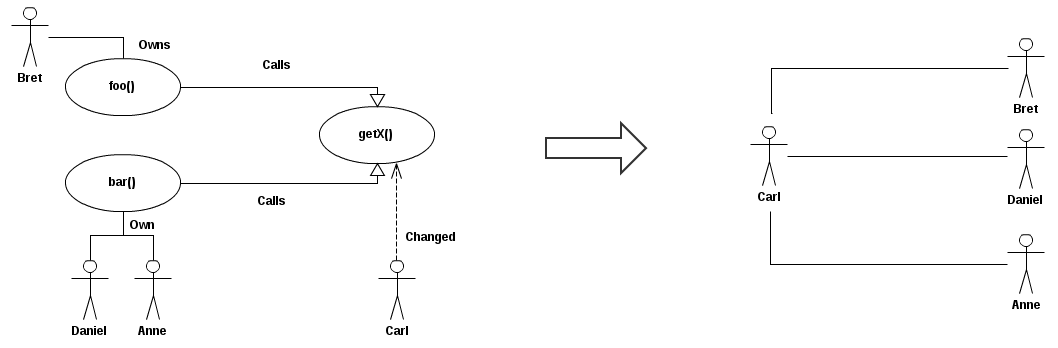
\includegraphics[width=0.9\textwidth]{images/TecNetwork}
\caption{A technical network for a code change. Carl has changed method getX() which is being
called by Bret's method foo() as well as Daniel and Anne's method bar().\label{fig:network}}
\end{figure*}

\section{Technical Approach}

\subsection{Extracting Technical Networks}
% End goal
The basis of this approach is to create a technical network of developers based on method ownership
and those method's call hierarchies effected by code changes. These networks will provide
dependency edges between contributors caused by code changes which may be 
identified as possible failure inducing pairings (Figure~\ref{fig:network}). To achieve this goal,
developer owners of methods, method call hierarchies (technical
dependencies) and code change effects on these hierarchies must be identified.
This approach is described in detail by illustrating its application to mining the data in a Git
repository although it can be used with any software repository.

% Owners
To determine which developers own which methods at a given code change,
the Git repository is queried. Git stores developers of a file per line, which was is to extrapolate
a percentage of ownership given a method inside a file.

% Call Graph
A method call graph is then constructed to extract method call hierarchies in a project at a given code change. 
Unlike other approaches such as Bodden's et al.~\cite{Bodden:2003:HVJ} 
of using byte code and whole projects, call graphs are built directly from source code files
inside of a code change, 
which does not have the assumptions of being able to compile or have access to all project 
files. It is important to not require project compilation at each code change because it is
an expensive operation as well as code change effects may cause the project
to be unable to compile. Using source files also allowed an update to the call graph
with changed files as opposed to completely rebuilding at 
every code change. This creates a rolling call graph which 
is used to show method hierarchy at each code change inside a project opposed to
a static project view.

% Changeset effects
The code change effect, if any, to the call hierarchy is now found. The Git
software repository is used to determine what changes were made to any give file inside a 
code change. Specifically, methods modified by a code change are searched for. The call graph 
is then used to determine which methods call those that have been changed, which
gives the code change technical dependencies.

%Resulting network
These procedures result in a technical network based on contributor method ownership 
inside a call hierarchy effected by a code change (Figure~\ref{fig:network} left hand side).
The network is then simplified by only using edges between developers, since the results
are only interested in discovering the failure inducing edges between developers and not the 
methods themselves (Figure~\ref{fig:network} right hand side). This is the final technical 
network.

\subsection{Identifying Failure Inducing Developer Pairs}
To identify failure inducing developer pairs (edges) inside technical networks, 
edges in relation to discovered code change failures are now analysed. To determine whether a code change 
was a success or failure (introduce a software failure), the approach of
Sliwerski et al.~\cite{Sliwerski:2005:CIF} is used. The following steps are then taken:

\begin{enumerate}
\item Identify all possible edges from the technical networks.
\item For each edge, count occurrences in technical networks of failed code changes.
\item For each edge, count occurrences in technical networks of successful code changes.
\item Determine if the edge is related to success or failure.
\end{enumerate}

To determine an edge's relation to success or failure,  the value FI (failure
index) which represents the normalized chance of a code change failure in the presence
of the edge, is created. 

\begin{equation}
\text{FI} = \frac{ \text{edge}_{failed} / \text{total}_{failed}}{\text{edge}_{failed} / \text{total}_{failed} + \text{edge}_{success} / \text{total}_{success}}
\end{equation}

Developer pairs with the highest FI value are said to be failure inducing structures
inside a project. These edges are stored in Table~\ref{tab:ratio}. A Fisher Exact Value test 
is also preformed on edge appearance in successful and failed
code changes, and non-appearance in successful and failed code changes to only
consider statistically significant edges. 


\section{Results}
To Illustrate the use of the approach, I conducted a case study of
the Hibernate-ORM project, an open source Java 
application hosted on GitHub\footnote{https://github.com/} with issue tracking 
performed by Jira\footnote{http://www.atlassian.com/software/jira/overview}.

This project was chosen because the tool created only handles Java code and it is written in Java 
for all internal structures and control flow
and uses Git for version control. Hibernate-ORM also uses issue tracking software which 
is needed for determining code change success or failure~\cite{Sliwerski:2005:CIF}.

In Hibernate-ORM, 27 statistically significant failure inducing developer pairs (A FI value of 0.5 or higher) 
were found out of a total of 46 statistically significant pairs that existed over the project's lifetime.
The pairings are ranked by their respective FI values (Table~\ref{tab:ratio}).

\begin{table}[h]
\begin{center}
\begin{tabular}{@{\hspace{.2cm}}ccc@{\hspace{.75cm}}c@{\hspace{.2cm}}c@{\hspace{.2cm}}}
\hline
Pair & Successful & Failed & FI & P-Value\\
\hline
(Daniel, Anne)	&	0&	14&	1.0000& 0.0001249		\\
(Carl, Bret)	&	1&	12&	0.9190& 0.003468	\\
(Emily, Frank)	&	1&	9&	0.8948& 0.02165      \\
\hline
\end{tabular}
\end{center}
\caption{The top 3 failure inducing developer pairs found and ordered by FI.\label{tab:ratio}}
\end{table}


\section{Conclusion and Future Work}
Technical dependencies are often used to predict software failures
in large software system~\cite{Pinzger:2008:DNP, Zimmermann:2008:PDU, Kim:2006:AIB}. 
This paper has presented a method for detecting failure inducing pairs of developers inside
of technical networks based on code changes. These developer pairs can be used in the prediction
of future bugs as well as provide coordination recommendations for developers within a project.

In future work, the adding of communication networks on a per code change basis is planned. In this,
the investigation of social and technical congruence on these networks and its effects on
software quality will be studied.



\bibliographystyle{IEEEtran}
\bibliography{paper}


% End of the paper
\end{document}
